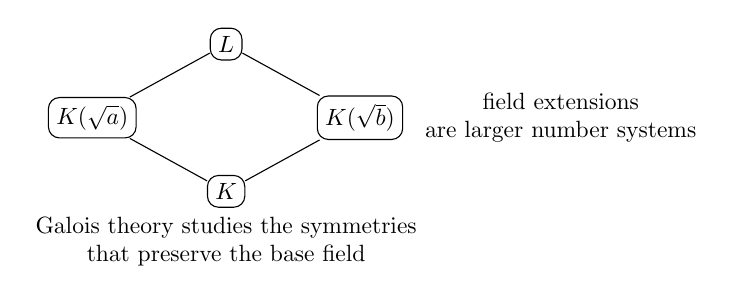
\begin{tikzpicture}[scale=.85,transform shape]
\node[draw,rounded corners] (top) at (2,2.2) {$L$};
\node[draw,rounded corners] (a) at (0,1.1) {$K(\sqrt a)$};
\node[draw,rounded corners] (b) at (4,1.1) {$K(\sqrt b)$};
\node[draw,rounded corners] (base) at (2,0) {$K$};
\draw (base)--(a)--(top)--(b)--(base);
\node[align=center] at (7,1.1) {field extensions\\are larger number systems};
\node[align=center] at (2,-.75) {Galois theory studies the symmetries\\that preserve the base field};
\end{tikzpicture}
